\documentclass{rapportECL}
\usepackage{lipsum}
\usepackage{svg}
\usepackage{algorithm}
\usepackage{algorithmic}
\usepackage{longtable}
\usepackage{subcaption} 
\usepackage[utf8]{inputenc}
\usepackage{ragged2e}   


\title{Rapport ECL - Template} %Titre du fichier

\begin{document}

%----------- Informations du rapport ---------

\titre{Implémentation d'Algorithmes pour les Systèmes d'Argumentation Abstraits} %Titre du fichier .pdf
\UE{Représentation des Connaissances et Raisonnement} %Nom de la UE
\sujet{ Introduction à l’Argumentation - Projet} %Nom du sujet

\enseignant{Elise \textsc{Bonzon}} %Nom de l'enseignant

\eleves{Hugo \textsc{Convert} \\
		Kiswendsida \textsc{OUEDRAOGO} } %Nom des élèves

%----------- Initialisation -------------------
        
\fairemarges %Afficher les marges
\fairepagedegarde %Créer la page de garde
\tabledematieres %Créer la table de matières

%------------ Corps du rapport ----------------
\begin{abstract}
	Ce rapport présente le travail réalisé dans le cadre du développement d’un outil dédié à la résolution de problèmes 
	dans le domaine des systèmes d’argumentation abstraits. Nous avons commencé par une exploration des algorithmes de 
	calcul des extensions complètes et stables, en nous appuyant sur des travaux de recherche sur l’argumentation. Ces 
	algorithmes ont été décrits, accompagnés d’explications sur leurs mécanismes et les structures 
	de données utilisées pour leur implémentation.

    Sur la base de ces algorithmes, nous avons pu répondre aux problématiques posées dans le sujet du projet, telles que la détermination 
	des extensions d’un système d’argumentation donné et l’évaluation de l’appartenance d’un argument à une extension.

    En complément, une interface graphique permettant de visualiser les systèmes d’argumentation, 
	leurs arguments, et les relations entre eux, a été développer pour faciliter l’analyse des résultats. 
\end{abstract}

\newpage % Crée une nouvelle page après l'abstract


\section{Introduction} 
Ce projet a nécessité une revue de littérature, au cours de laquelle nous avons identifié des ressources clés pour notre travail.


Tout d'abord, le cours d'Élise Bonzon sur l'argumentation computationnelle \cite{a} nous a offert une base pour appréhender les concepts fondamentaux. 
Ensuite l'article \textit{An Introduction to Argumentation Semantics} \cite{b}, qui propose des définitions assez approfondies des différentes sémantiques de l'argumentation. 
Enfin, l’étude des algorithmes pour les sémantiques d'argumentation, présentée dans \textit{Algorithms for Argumentation Semantics: Labeling Attacks as a Generalization of Labeling Arguments} \cite{c}, 
nous a permis d’approfondir nos connaissances sur les algorithmes utilisés dans ce domaine et ainsi implémenter la solution du projet présent. 


Ces travaux de référence ont guidé notre démarche et orienté la définition des objectifs ainsi que des fonctionnalités attendues, conformément aux directives de l'énoncé.

\section{Objectifs et fonctionnalités attendues du projet}
Ce projet à pour objectif la mise en place d'une solution destiné à résoudre des problèmes spécifiques liés aux systèmes d'argumentation abstraits (AF). 
Un système d'argumentation est défini par un ensemble d'arguments (A) et d’un ensemble de relations d'attaque (R) entre ces arguments. 
L’enjeu principal est donc de concevoir l'outil capable pour identifier les extensions complètes et stables, tout en évaluant l’appartenance d’un argument données à ces extensions, selon des critères crédibles ou sceptiques.


Le programme est conçu pour lire un système d'argumentation à partir d’un fichier texte formaté, analyser les données et produire des résultats conformes à la sémantique utilisée. Initialement prévu pour fonctionner en mode console, il a été enrichi par l’ajout d’une interface graphique
\section{Algorithmes et structures de données} 


\subsection{Algorithmes}
Les algorithmes utilisés pour l'implémentation de ce projet sont spécifiquement ceux dédiés à l'énumération des extensions complètes 
et stables. Ces algorithmes sont issus des travaux présentés dans l'article 
\textit{"Algorithms for Argumentation Semantics: Labeling Attacks as a Generalization of Labeling Arguments"} \cite{c}.
Les deux algorithmes présentés ci-dessous s’appuient sur l’utilisation d’étiquettes qui sont IN, OUT,  {MUST\_OUT}, BLANK et UNDEC.
{MUST\_OUT} et BLANK, qui n’ont pas été abordés en cours, peuvent être considérés ici comme des détails propres à l’implémentation.

L'étiquette {IN} identifie les arguments qui peuvent appartenir à  l'extension recherchée. L'étiquette {OUT} 
identifie un argument qui est attaqué par un argument {IN}. L'étiquette {BLANK} est attribuée à tout argument non 
traité dont l'étiquette finale n'est pas encore déterminée. L'étiquette {MUST\_OUT} identifie les arguments qui attaquent des 
arguments {IN}. Enfin, l'étiquette {UNDEC} désigne les arguments qui pourraient ne pas être inclus dans  l'extension, car ils pourraient ne pas être défendus par un argument {IN}.


\begin{itemize}
    \item Énumération des extensions stables.
    
	L'algorithme ci-dessous identifie toutes les extensions stables d’un AF $(A, R)$ \cite{c} (p. 642). %\cite{ref}  
	On remarque l'absence d'utilisation du label {UNDEC}. La sémantique du label {MUST\_OUT} peut être interprétée comme celle 
	d'un {UNDEC} mais attaquant un argument étiqueté \({IN}\). 
	Cependant, dans une labellisation visant à identifier une extension stable, aucun argument ne devrait rester étiqueté {UNDEC} à 
	la fin. 

	Le label {MUST\_OUT} est utilisé pour désigner les arguments attaquant des label {IN} et susceptibles d'évoluer 
	vers {OUT} à la fin de la labellisation. Ainsi, un ensemble d'arguments \( S \), étiqueté \({IN}\), est 
	considéré comme stable uniquement s'il n'existe aucun argument étiqueté {MUST\_OUT} à l'issue d'une labellisation de tous les Arguments.

	\begin{algorithm}
		\caption{Enumerating all stable extensions of an AF $(A, R)$}
		\begin{algorithmic}[1]
			\STATE $Lab : A \to \{IN, OUT,  MUST\_OUT, BLANK\}$; $Lab \gets \emptyset$
			\FORALL{$x \in A$}
				\STATE $Lab \gets Lab \cup \{(x, BLANK)\}$
			\ENDFOR
			\STATE $Estable \subseteq 2^A$; $Estable \gets \emptyset$
			\STATE \textbf{call} find-stable-extensions($Lab$)
			\STATE \textbf{report} $Estable$ is the set of all stable extensions
			\STATE \textbf{procedure} find-stable-extensions($Lab$)
			\WHILE{there exists $y \in A$ such that $Lab(y) = BLANK$}
				\IF{there exists $y$ such that $Lab(y) = BLANK$ and $\forall z \in \{y\}^- : Lab(z) \in \{OUT,  MUST\_OUT\}$}
					\STATE select $y$ such that $Lab(y) = BLANK$
				\ELSE
					\STATE select $y$ such that $Lab(y) = BLANK$ and $\forall z : Lab(z) = BLANK$, 
					\STATE $\left| \{x : x \in {y}^+ \land Lab(x) \neq OUT \} \right| \geq \left| \{x : x \in {z}^+ \land Lab(x) \neq OUT \} \right|$
				\ENDIF
				\STATE $Lab' \gets Lab$
				\STATE $Lab'(y) \gets IN$
				\FORALL{$z \in {y}^+$}
					\STATE $Lab'(z) \gets OUT$
				\ENDFOR
				\FORALL{$z \in {y}^-$}
					\IF{$Lab'(z) = BLANK$}
						\STATE $Lab'(z) \gets  MUST\_OUT$
					\ENDIF
					\IF{for all $w \in {z}^-$, $Lab'(w) \neq BLANK$}
						\STATE $Lab(y) \gets  MUST\_OUT$
					\ENDIF
				\ENDFOR
				\STATE \textbf{goto} line 7
				\STATE \textbf{call} find-stable-extensions($Lab'$)
				\IF{there exists $z \in {y}^-$ such that $Lab(z) = BLANK$}
					\STATE $Lab(y) \gets  MUST\_OUT$
				\ELSE
					\STATE $Lab \gets Lab'$
				\ENDIF
				\IF{for all $x$, $Lab(x) \neq  MUST\_OUT$}
					\STATE $S \gets \{x : Lab(x) = IN\}$
					\STATE $Estable \gets Estable \cup \{S\}$
				\ENDIF
			\ENDWHILE
		\end{algorithmic}
	\end{algorithm}
	\begin{quote}
$(y, z) \in R$ signifie que $y$ attaque $z$ (ou que $z$ est attaqué par $y$).  
On note $\{y\}^-$ l'ensemble des arguments qui attaquent $y$,  
et $\{y\}^+$ l'ensemble des arguments attaqués par $y$.  
	\end{quote}	


Le processus commence par l'initialisation des arguments avec un label  {BLANK}, signifiant qu'aucun argument n'a encore été catégorisé. 
Ensuite, l'algorithme cherche à trouver toutes les extensions stables possibles en étiquetant les arguments de manière appropriée. 
Tant qu'il existe des arguments non étiquetés, l'algorithme sélectionne un argument \( y \) avec un label  {BLANK}. 
Le critère de sélection dépend de la situation : si l'argument \( y \)  est {BLANK} avec ses attaquants  {OUT} ou {MUST\_OUT}, il est selectionné pour être labellisé {IN}. 
Dans le cas contraire, l'algorithme choisit un argument \( y \) de manière à maximiser le nombre d'arguments attaqués par \( y \) (l'ensemble \( {y}^+ \)) qui ne sont pas encore étiquetés \( {OUT} \).


Une copie  de l'état des labels est effectuée pour une première propagation des étiquettes (Lab' <- Lab).


Les éléments de l'ensemble \( \{y\}^+ \)) reçoivent le label  {OUT}, indiquant qu'ils sont exclus de l'extension, car attaqué par y. 
Les arguments voisins attaquant \( y \) correspondant aux éléments de \( \{y\}^- \) mais qui ne sont pas encore traités ({BLANK}) reçoivent le label {MUST\_OUT}, ils doivent être exclus et ne peuvent pas faire partie de l'extension. 

Si l'argument \( z \), qui était jusqu'à présent non traité, a tous ses attaquants déjà étiquetés autre que \texttt{BLANK}, 
cela entraîne la mise à jour du label de \( y \) en \texttt{MUST\_OUT}. En effet, cela signifie que \( y \) devient incompatible 
avec l'extension en cours. Dans ce cas, on effectue un retour anticipé au début de la boucle.


Une fois que les labels ont été modifiés, l'algorithme procède à une exploration récursive en appelant à nouveau la procédure pour tester de nouvelles configurations. 

On s'assure qu'il n'existe aucun argument \( z \) dans l'ensemble \( \{y\}^- \) qui soit étiqueté \(  {BLANK} \) dans l'état \( Lab \). Si tel est le cas, l'argument \( y \) est étiqueté \(  {MUST\_OUT} \). Sinon, l'état \( Lab \) est mis à jour pour être égal à l'état tampon \( Lab' \).

Si tous les arguments attaqués par \( y \) ont des labels autres que  { MUST\_OUT}, l'extension est considérée comme stable et l'ensemble des arguments étiquetés  {IN} est ajouté à l'ensemble des extensions stables.

L'exécution du bloc suivant l'appel récursif est mise dans la pile d'exécution, et elle sera traitée après tous les appels récursifs.

\newpage

\item Énumération des extensions complètes.


L'algorithme ci dessous de identifie toutes les extensions complètes d’un AF (A,R) \cite{c} (p.644).

\begin{algorithm}
    \caption{Enumerating all complete extensions of an AF $(A, R)$}
    \begin{algorithmic}[1]
        \STATE $Lab : A \to \{\text{IN}, \text{OUT}, \text{MUST\_OUT}, \text{UNDEC}, \text{BLANK}\}$; $Lab \gets \emptyset$
        \FORALL{$x \in A$}
            \STATE $Lab \gets Lab \cup \{(x, \text{BLANK})\}$
        \ENDFOR
        \STATE $E_{\text{complete}} \subseteq 2^A$; $E_{\text{complete}} \gets \emptyset$
        \STATE \textbf{call} find-complete-extensions($Lab$)
        \STATE \textbf{report} $E_{\text{complete}}$ is the set of all complete extensions
        \STATE \textbf{procedure} find-complete-extensions($Lab$)
        \IF{there exists $y \in A$ such that $Lab(y) = \text{MUST\_OUT}$}
            \RETURN
        \ENDIF
        \IF{for all $x \in A$, $Lab(x) \in \{\text{UNDEC}, \text{BLANK}\} \implies \forall z \in \{x\}^-, Lab(z) = \text{OUT}$}
            \STATE $S \gets \{w \in A \mid Lab(w) = \text{IN}\}$
            \STATE $E_{\text{complete}} \gets E_{\text{complete}} \cup \{S\}$
        \ENDIF
        \WHILE{there exists $y \in A$ such that $Lab(y) = \text{BLANK}$}
            \IF{$\forall z \in \{y\}^-, Lab(z) \in \{\text{OUT}, \text{MUST\_OUT}\}$}
                \STATE select $y$ such that $Lab(y) = \text{BLANK}$
            \ELSE
                \STATE select $y$ such that $Lab(y) = \text{BLANK}$ and $\forall z : Lab(z) = \text{BLANK}$,
                \STATE $\left| \{x \mid x \in {y}^+ \land Lab(x) \neq \text{OUT} \} \right| \geq \left| \{x \mid x \in {z}^+ \land Lab(x) \neq \text{OUT} \} \right|$
            \ENDIF
            \STATE $Lab' \gets Lab$
            \STATE $Lab'(y) \gets \text{IN}$
            \FORALL{$z \in {y}^+$}
                \STATE $Lab'(z) \gets \text{OUT}$
            \ENDFOR
            \FORALL{$z \in {y}^-$}
                \IF{$Lab'(z) \in \{\text{UNDEC}, \text{BLANK}\}$}
                    \STATE $Lab'(z) \gets \text{MUST\_OUT}$
                \ENDIF
                \IF{for all $w \in {z}^-, Lab'(w) \neq \text{BLANK}$}
                    \STATE $Lab(y) \gets \text{UNDEC}$
                \ENDIF
            \ENDFOR
            \STATE \textbf{goto} line 7
            \STATE \textbf{call} find-complete-extensions($Lab'$)
            \IF{there exists $z \in {y}^-$ such that $Lab(z) \in \{\text{BLANK}, \text{UNDEC}\}$}
                \STATE $Lab(y) \gets \text{UNDEC}$
            \ELSE
                \STATE $Lab \gets Lab'$
            \ENDIF
        \ENDWHILE
    \end{algorithmic}
\end{algorithm}

 L'algorithme 2 repose sur le même principe que le préccédent avec quelques petits changements pour satisfaire les conditions d'extension stable.
 On part toujours sur la base d'arguments tous etiquettés à blanc;  le critère de selection d'argument pour la propagation des labels reste le même.
 On remarque l'utilisation du label UNDEC ici pour indiquer une indécision, alors que cette situation avait immédiatement été 
 rejetée dans l'algorithme 1 en tant qu'incompatibilité, en la plaçant sous le label MUST\_OUT.

 
 on détermine si un ensemble \( S \) (les éléments dont le label est \( \text{IN} \)) est une extension complète en vérifiant 
 deux conditions. 

 	\begin{enumerate}
		\item Tout d'abord, garantir qu' aucun élément \( x \) de \( A \) n'est marqué 
		comme \( \text{MUST\_OUT} \).
		\item Ensuite, on vérifie qu'il n'existe pas un élément \( z \) 
		qui reste indéterminé (\( \text{UNDEC} \) ou \( \text{BLANK} \)) et qui aurait tous ses attaquants (les éléments de \( \{z\}^- \)) déjà marqués  \( {OUT} \).
	\end{enumerate}

\end{itemize}

\newpage

\subsection{structures de données}

La manipulation des données dans le projet repose essentiellement sur l’utilisation de listes et de dictionnaires pour la représentation des arguments et des relations d’attaque.

\begin{itemize}
    \item Les arguments sont stockés dans une liste ou un ensemble. Par exemple : 
    \[
    {arguments = \{'A', 'B', 'C'\}}
    \]
    où \( A \), \( B \) et \( C \) représentent les arguments.

    \item Les attaques sont représentées par un dictionnaire, chaque clé correspondant à un argument et la valeur étant l’ensemble des arguments qu’il attaque. Par exemple :
    \[
    {attacks = \{'A': \{'B', 'C'\}, 'B': \{'C'\}\}}
    \]
    Ici, \( A \) attaque \( B \) et \( C \), tandis que \( B \) attaque \( C \).
\end{itemize}


\section{Implémentation et tests}

\subsection{Implémentation}

La proposition de solution a été faite \textbf{Python}. Nous avons choisi Python pour sa simplicité d'implémentation et sa flexibilité pour la manipulations des structures 
de données  telles que les listes et les dictionnaires que nous utilisons.

\subsubsection{Architecture}

L'architecture du projet repose sur l'utilisation de classes et de méthodes afin de faciliter le partage des données et des fonctions entre différents composants répartis sur plusieurs fichiers. Les principales parties de l'architecture sont décrites ci-dessous :

\begin{itemize}
    \item \textbf{main.py} : Ce fichier sert de point d'entrée principal pour l'exécution de la solution. L'utilisateur peut lancer le programme en mode console avec les paramètres suivants :
    \begin{itemize}
        \item \texttt{-P} : pour spécifier la sémantique de calcul.
        \item \texttt{-f} : pour indiquer le fichier contenant l'Argumentation Framework (AF).
        \item \texttt{-a} : (optionnel) pour spécifier les arguments, en fonction de la sémantique choisie.
    \end{itemize}
    Ce fichier appelle les autres fichiers pour le traitement des données et l'exécution des algorithmes, parmi lesquels on a:

    \item \textbf{utilities.py} : Ce fichier contient des classes et des méthodes utilitaires, comme la classe \texttt{file\_reader}, qui permet de lire les fichiers contenant l'AF. Ces méthodes facilitent la gestion des fichiers et la manipulation des données avant leur traitement.

    \item \textbf{controller.py} : Ce fichier contient les méthodes responsables de la gestion des flux de données. Il fait appel aux méthodes de calcul spécifiques en fonction des paramètres fournis par l'utilisateur, en organisant et en contrôlant l'exécution des algorithmes.

    \item \textbf{computing\_methods.py} : Ce fichier contient l'implémentation des algorithmes d'énumération des extensions complètes et stables. Afin de garantir une bonne lisibilité du code, les parties répétitives dans les algorithmes ont été extraites et regroupées dans des méthodes uniques. Par exemple, la méthode \texttt{select\_argument} est utilisée pour sélectionner un argument dans les différents algorithmes afin de réduire la duplication du code.

    \item \textbf{af\_visualizer.py} : Ce fichier gère l'interface graphique de l'application. Il est basé sur les mêmes méthodes des fichiers précédemment mentionnés, permettant une interaction visuelle avec l'utilisateur pour soumettre des fichiers et afficher les résultats sous une forme graphique.

\end{itemize}

\subsection{Tests et validation}

Pour vérifier l'exactitude de notre implémentation des algorithmes d'énumération des extensions stables et complètes, nous avons réalisé des tests sur plusieurs frameworks argumentatifs. Dans le tableau dessous nos recensons les résultats de quelques tests. 
Les fichiers de test, au format .apx, se trouvent dans un répertoire "tests" au sein du projet. Ces fichiers sont reçus en entrée, car ils contiennent la description des systèmes d'argumentation abstraits (AF).
\vspace{0.5cm}
\noindent


\begin{longtable}{|p{7cm}|p{7cm}|}
	\hline
	\textbf{Commande exécutée} & \textbf{Résultats (console et interface graphique)} \\ 
	\hline
	\endfirsthead
	\hline
	\textbf{Commande exécutée} & \textbf{Résultats (console et interface graphique)} \\ 
	\hline
	\endhead
	\hline
	\endfoot
	

	\texttt{python .\textbackslash main.py -p SE-CO -f .\textbackslash tests\textbackslash test\_af2.apx} & 
	\begin{minipage}{\linewidth}
		\centering
		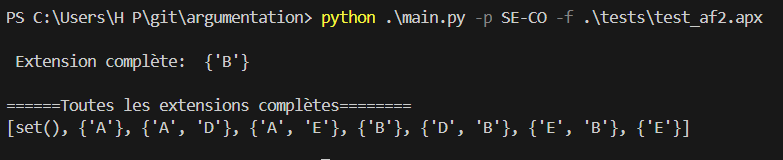
\includegraphics[width=\linewidth]{img/a_consol.png} \\[0.2cm]
		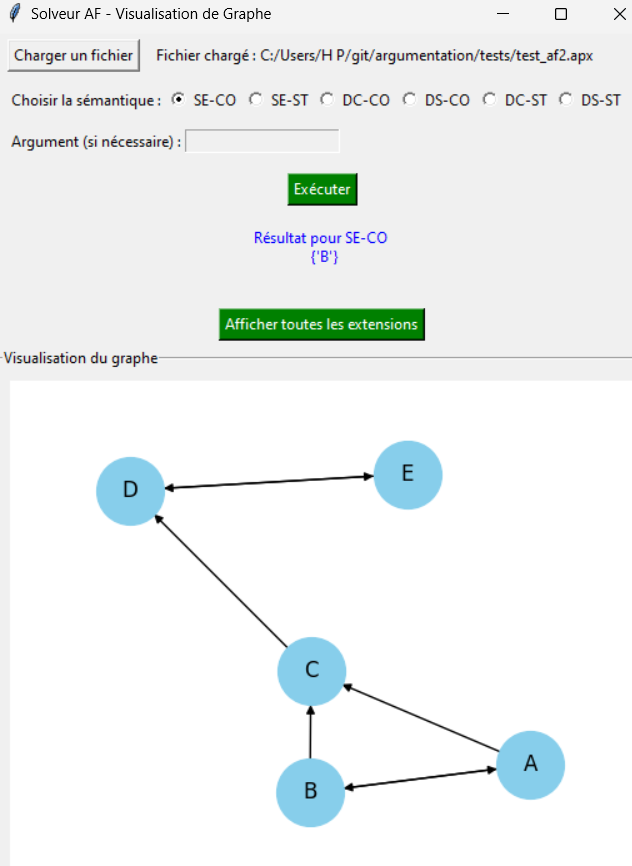
\includegraphics[width=\linewidth]{img/a_ui.png}
	\end{minipage} \\[0.2cm]

	
	\hline
	\texttt{python .\textbackslash main.py -p DC-CO -f .\textbackslash tests\textbackslash test\_af2.apx -a 'B'} & 
	\begin{minipage}{\linewidth}
		\centering
		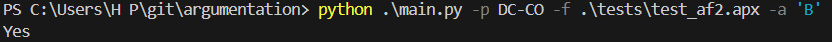
\includegraphics[width=\linewidth]{img/b_consol.png} \\[0.2cm]
		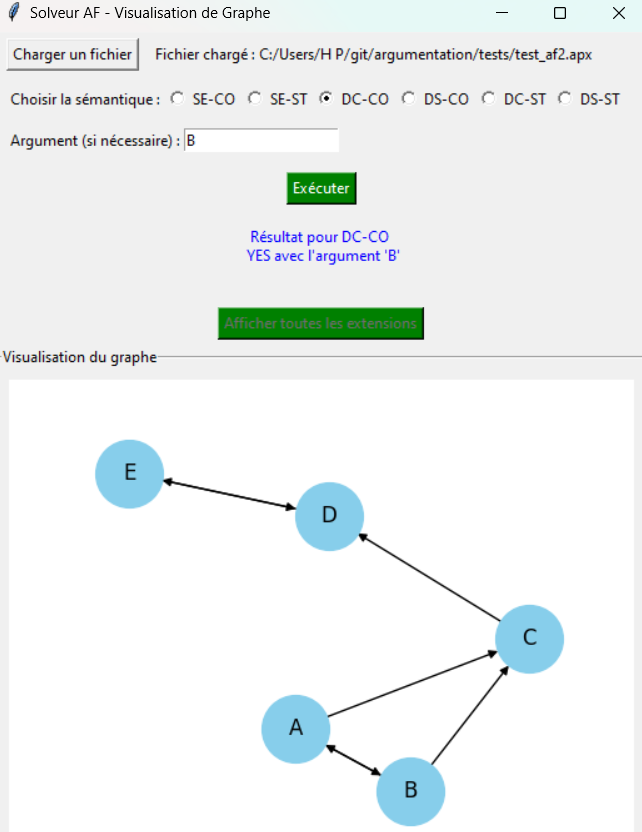
\includegraphics[width=\linewidth]{img/b_ui.png}
	\end{minipage} \\[0.2cm] \\
	\hline


	\texttt{python .\textbackslash main.py -p SE-ST -f .\textbackslash tests\textbackslash test\_af4.apx} & 
	\begin{minipage}{\linewidth}
		\centering
		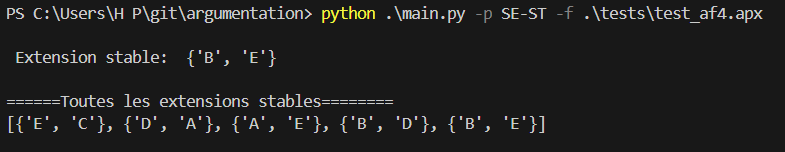
\includegraphics[width=\linewidth]{img/c_consol.png} \\[0.2cm]
		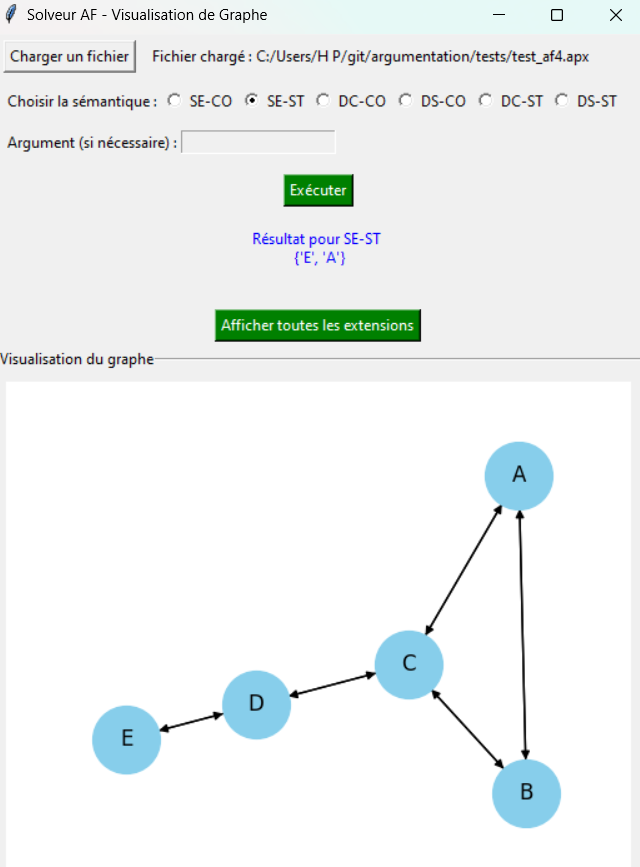
\includegraphics[width=\linewidth]{img/c_ui.png}
	\end{minipage} \\[0.2cm] \\
	\caption{La commande pour lancer l'interface graphique est \texttt{python af\_visualizer.py}.}

	\end{longtable}




\vspace{0.5cm}
\noindent

Les résultats de nos tests confirment le bon fonctionnement de notre implémentation des algorithmes. Les extensions calculées correspondent aux attentes théoriques pour chaque cas testé, validant ainsi l'exactitude de notre implémentation.

\subsubsection{Remarque sur les fichiers de test.} 
Dans le cadre des tests réalisés, nous avons constaté une petite disparité dans les formats des fichiers fournis. En effet, alors que les spécifications de l'énoncé imposaient que chaque ligne décrivant un argument ou une attaque se termine par un point (par exemple, \texttt{arg(a).} ou \texttt{att(a,b).}), certains fichiers de test présentaient des lignes sans point final, comme \texttt{arg(a)} ou \texttt{att(a,b)}. Afin de garantir une compatibilité avec ces fichiers, notre implémentation a été adaptée pour gérer les deux formats. 


\section{Conclusion}
En conclusion, ce projet a été l'occasion d'élargir nos connaissances sur les systèmes d'argumentation abstraits, 
à travers une revue de littérature et l'implémentation pratique d'algorithmes d'énumération d'extensions. 

L'intégration de ces algorithmes dans un outil fonctionnel a permis de concrétiser notre apprentissage. 
Ce travail constitue une contribution à l'application des théories de l'argumentation et ouvre la voie à des perspectives d'amélioration.



\bibliographystyle{unsrt} 
\bibliography{mybib}

\end{document}
